\section{User Interface}
\subsection{Description}
When the sensor data has arrived at the remote PC, the data has to be read out. The data should be at least be output to a console. If possible due to time constraints, the data will be more visualised.
\subsubsection{CUI}
The CUI (Console User Interface) is the most basic way the data will be output. All the sensor data will be output to the control with corresponding label. In order to make the CUI readable, it will be possible to filter the data and control the refresh rate of the data.
\begin{figure}[H]
	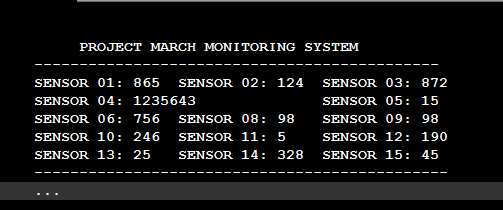
\includegraphics{MockupCUI}
\end{figure} 
\subsubsection{GUI}
\subsection{Framework}
In order to choose a language, there are two important factors in this project which have to be taken in account. Firstly, the framework should have a rich support of visualising data. Secondly, the framework must be able to support 3D rendering. Keeping this in mind, the options of languages are narrowed down to C/C++, Java \& Python because these are known to have a rich selection of libraries which support 3D rendering and data visualisation. In addition, since SimuLink is a MatLab module, using MatLab as framework is also an option. 
\subsubsection{MatLab}
\subsection{3D-Rendering}
Because of the fact that the 3d-rendering has shifted to a lower priority, less effort has been expended in researching suitable frameworks for rendering. Still, a small list have been compiled of some rendering frameworks which are simple to use for each of the narrowed down languages.
\begin{itemize}
	\item C/C++: Ogre3D
	\item Java/Scala: Env3D
	\item Python: Panda3D
\end{itemize}
